\documentclass[9pt,twoside]{pnas-new}
\setboolean{displaywatermark}{false}
\setlength{\textfloatsep}{6pt plus 1pt minus 2pt}
\setlength{\floatsep}{5pt plus 1pt minus 2pt}
\setlength{\intextsep}{5pt plus 1pt minus 2pt}
% Paste this file into the PNAS single-column mathematics article template on Overleaf.
% Upload the local paper_overleaf/figures folder as figures/ in the Overleaf project.
% The PNAS template support files should remain in the Overleaf project.

\articletype{Research Article}
\templatetype{pnasmathematics}

\begin{document}

\title{Pitcher-specific state machines predict Major League Baseball pitch selection}

\author[a,1]{David Adkins}

\affil[a]{Department of Quantitative Social Science, Dartmouth College, Hanover, NH}

\leadauthor{Adkins}

\significancestatement{Baseball pitch selection is a compact example of strategic sequential decision-making. A pitcher repeatedly chooses among a small set of actions while accounting for count, batter handedness, previous pitches, game context, and personal repertoire. This project models that process for 100 Major League Baseball pitchers using interpretable state machines, ordinary least squares regressions, gradient-boosted classifiers, XGBoost, SHAP explanations, and a stacked ensemble. The results show that simple context-dependent state probabilities explain a substantial share of pitch choice, while boosted models add predictive accuracy by learning nonlinear interactions among pitcher identity, current-game behavior, recent-start tendencies, and batter matchup history.}

\authorcontributions{D.A. designed the study, assembled the data pipeline, implemented the statistical models, generated the visualizations, and wrote the manuscript.}
\authordeclaration{The author declares no competing interests.}
\equalauthors{}
\correspondingauthor{\textsuperscript{1}To whom correspondence should be addressed. E-mail: david.adkins.26@dartmouth.edu}
\keywords{baseball analytics $|$ state machines $|$ gradient boosting $|$ SHAP $|$ pitch sequencing}

\begin{abstract}
Pitch selection in baseball is observable at high frequency but only partly predictable. Each pitch is chosen from a pitcher-specific arsenal under changing count, batter, and game conditions. This project asks whether the next pitch thrown by Major League Baseball pitchers can be modeled as a probabilistic state process and whether modern machine-learning models add reliable accuracy beyond that state structure. Using Statcast pitch-level data for the top 100 pitchers by 2025 pitch volume, I construct sequence features for 261,620 pitches from March 18 through September 28, 2025, and evaluate temporal generalization on 82,282 pitches from the same pitcher pool observed from March 25 through June 4, 2026. A smoothed pitcher-count-previous-pitch-batter-side state machine attains 42.3\% exact accuracy and 84.2\% top-three accuracy on a held-out 2025 split. A recency-weighted stacked model combining histogram gradient boosting, XGBoost, and state-machine probabilities improves exact accuracy to 44.1\% on the 2025 holdout and 40.4\% on the 2026 validation set. OLS coefficient surfaces and grouped SHAP explanations show that pitcher arsenal, previous pitch type, count leverage, batter handedness, and recent usage history are the main information sources. The results support a conservative conclusion: pitch choice is not deterministic, but it is structured enough for interpretable state models and boosted classifiers to recover meaningful strategic regularities.
\end{abstract}

\dates{This manuscript was compiled on \today}
\doi{\url{www.pnas.org/cgi/doi/10.1073/pnas.XXXXXXXXXX}}

\maketitle
\thispagestyle{firststyle}
\ifthenelse{\boolean{shortarticle}}{\ifthenelse{\boolean{singlecolumn}}{\abscontentformatted}{\abscontent}}{}

\Firstpage

\section*{Introduction and related work}

Pitch calling is one of baseball's clearest repeated decision problems. A pitcher does not choose from the entire vocabulary of baseball pitches. He chooses from his own repertoire or "arsenal" against a particular batter, in a particular count, after a sequence of prior pitches, with a game state that changes after almost every event. The same four-seam fastball can mean different things at 0--0, 0--2, and 3--2 counts. A slider may be a chase pitch after a fastball, but a liability after the hitter has already seen it twice. The question I pose is whether observed pitch choices contain enough regularity to be modeled as a state-dependent probability distribution.

This question sits inside a growing baseball analytics literature on pitch prediction. Hamilton et al. were among the earlier studies to frame next-pitch prediction as a supervised machine-learning problem, comparing different classification methods for predicting pitch type from game situation and pitch history \cite{hamilton2014pitch}. Sidle and Tran later compared multi-class classification methods for baseball pitch types and emphasized that real-time prediction depends on using features available before the pitch is thrown \cite{sidle2018multiclass}. Lee extended the problem by predicting both pitch type and pitch location with an ensemble of deep neural networks, showing that neural models can learn richer interactions across game state, pitcher tendencies, and batter context \cite{lee2022pitch}. More recent work by Lin and Wu compares machine-learning and deep-learning approaches for MLB pitch-type prediction, reflecting the broader shift from simple classifiers to flexible ensemble and neural architectures \cite{lin2025pitchtype}. Applied public-facing projects, such as Augustine's MLB pitch predictor, show that the same question has practical appeal beyond academic publications and continues to be debated among baseball fans and scouts \cite{augustine2024pitchpredictor}.

This project differs from much of the prior work in three ways. First, it places a  state machine at the center of the analysis rather than treating the model only as a classifier. The state machine asks a baseball-native question, which, in my experience, many baseball players ask themselves while at bat. This question is: given the pitcher, count, previous pitch, and batter side, what pitch menu has this pitcher historically used? Second, it evaluates whether boosted classifiers add information beyond that interpretable state structure. Third, it tests temporal generalization by training on 2025 data and evaluating on 2026 pitches from the same pitcher pool.

The project builds its model in a sequence of increasingly flexible specifications. The first specification is a state machine. For each pitcher and context, a state machine estimates the empirical probability of each pitch type, then use smoothing and fallback states when a context is sparse. The second specification uses ordinary least squares (OLS) linear probability models to summarize how count, prior pitch, batter side, and pitcher fixed effects shift the probability of specific pitch types. The third specification uses boosted decision-tree models, including histogram gradient boosting and XGBoost, to learn nonlinear interactions among pitcher identity, batter identity, pitch history, and game context. The final specification stacks the boosted models with the state-machine probabilities so that the final prediction can use both parametric learning and explicit sequence frequencies.

\section*{Data}

The analysis uses public Statcast pitch-level data collected through Baseball Savant \cite{baseballsavant}. Statcast data were accessed locally through the Python package \texttt{pybaseball}, which provides extensive access to public baseball data sources \cite{pybaseball}. The pybaseball package includes pitch-level data for MLB dating back to 2015, including pitch type, speed, result, and various other details about any particular pitch from 2015-2026. The training sample contains the top 100 pitchers by 2025 pitch volume and covers games from March 18 through September 28, 2025. The processed sequence table contains 261,620 pitch rows after removing rows without a pitch type and constructing lagged context. The temporal validation sample uses 2026 pitches thrown by the same 2025 pitcher pool from March 25 through June 4, 2026. Ninety-two of the 100 pitchers had usable 2026 observations during this window, producing 82,282 validation rows after alignment to the 2025 pitch-type vocabulary.

Each row represents the information available before an observed pitch is thrown. The target variable is the pitch type actually thrown. The core categorical predictors are pitcher name, batter name, batter side, pitcher throwing hand, count, base-out state, previous pitch type, pitch type two pitches ago, previous pitch result, and inning half. Numeric predictors include balls, strikes, outs, inning, pitch number, previous zone, previous release speed, previous plate location, score differential from the batting team's perspective, and lineup handedness shares. Additional engineered features summarize current-game pitch mix, pitcher-batter matchup history, batter history, pitcher history, and recent-start pitch mix over the previous three appearances.

The 2025 data are split chronologically enough to avoid using the 2026 validation sample during model fitting, but the main holdout comparison is a stratified 80/20 split within 2025. Within the 80\% development split, a second split is used to train the stacking model, which has base models that are trained on one portion, with their probabilities scored on a calibration portion, and a multinomial logistic regression stacker learns how to combine histogram gradient boosting, XGBoost, and state-machine probabilities. Final base models are then refit on the full development split before scoring the 2025 holdout and 2026 temporal validation set.

\section*{Methods}

\subsection*{State-machine model}

The state-machine model estimates a conditional distribution over pitch types. The primary state is pitcher, count, previous pitch type, and batter side. For a state $s$ and pitch type $p$, the smoothed estimate is
\begin{equation}
\Pr(p \mid s)=\frac{n_{s,p}+\alpha}{n_s+\alpha K},
\end{equation}
where $n_{s,p}$ is the number of training pitches of type $p$ observed in state $s$, $n_s$ is the number of pitches in that state, $K$ is the number of pitch classes, and $\alpha=1$ is Laplace smoothing. If a state has fewer than five training observations, the model backs off to less specific states, ending at the pitcher's overall pitch distribution. This is a finite-state approximation to a Markov process in which the next pitch depends on a compact representation of the recent state rather than the entire game history \cite{norris1998markov}.

\subsection*{OLS beta analysis}

OLS is used as a descriptive model, not as the strongest predictor. For major pitch outcomes, the dependent variable is an indicator that the observed pitch is a given pitch type. Predictors include count, previous pitch type, batter side, previous pitch result, and pitcher fixed effects. The resulting beta coefficients create two useful summaries. First, pitcher-by-pitch intercept surfaces show which pitchers are structurally more likely to throw each pitch type after accounting for context. Second, context beta surfaces show how counts and prior pitches shift pitch probabilities. This step connects the model to classical regression and makes the later boosted results easier to interpret \cite{wooldridge2010econometric}.

\subsection*{Boosted and stacked models}

The boosted models use histogram gradient boosting and XGBoost. Gradient boosting fits an additive sequence of decision trees, where later trees correct errors from earlier trees \cite{friedman2001greedy}. XGBoost uses a regularized tree-boosting objective with shrinkage, subsampling, and efficient tree construction \cite{chen2016xgboost}. In this project, XGBoost is configured with 220 estimators, maximum tree depth 4, learning rate 0.06, subsampling 0.90, column subsampling 0.90, L2 regularization 2.0, and L1 regularization 0.05. Histogram gradient boosting uses learning rate 0.08, 160 iterations, 31 maximum leaf nodes, and L2 regularization 0.05.

Both boosted models are trained with recency weights. If a pitch is $d$ days older than the most recent training pitch, its weight is proportional to $0.5^{d/45}$ and then normalized to mean one. This makes recent behavior more influential without discarding older observations. The stacked model then concatenates the class-probability vectors from histogram gradient boosting, XGBoost, and the state machine, and fits a multinomial logistic regression meta-model with $C=0.75$. All models are evaluated using exact accuracy, top-two accuracy, top-three accuracy, macro F1, average probability assigned to the actual pitch, model confidence, and log loss.

\subsection*{SHAP interpretation}

SHAP values are used to interpret feature importance in the boosted workflow \cite{lundberg2017unified}. Because one-hot encoded player names can dominate raw feature rankings, features are also grouped into baseball concepts such as pitcher identity and arsenal, previous pitch type, two-pitches-ago pitch type, count leverage, batter handedness, previous release speed, previous pitch result, base-out state, pitch number, and score differential. This grouped interpretation is more faithful to the baseball question because it reads player identity as a proxy for repertoire and role rather than as a standalone causal variable.

\section*{Results}

\subsection*{Model comparison}

The first result is that a simple state machine is already a strong predictor. On the 2025 holdout, a dummy baseline that predicts the most common eligible pitch reaches 31.9\% exact accuracy. The smoothed state machine raises exact accuracy to 42.3\% and top-three accuracy to 84.2\%. This improvement shows that count, previous pitch, batter side, and pitcher identity can reduce the plausible pitch set. The boosted models add further accuracy, and the stacked model performs best on exact accuracy in both evaluation periods. It reaches 44.1\% exact accuracy and 86.2\% top-three accuracy on the 2025 holdout, then 40.4\% exact accuracy and 82.1\% top-three accuracy on 2026 validation.

\begin{figure}[tbhp]
\centering
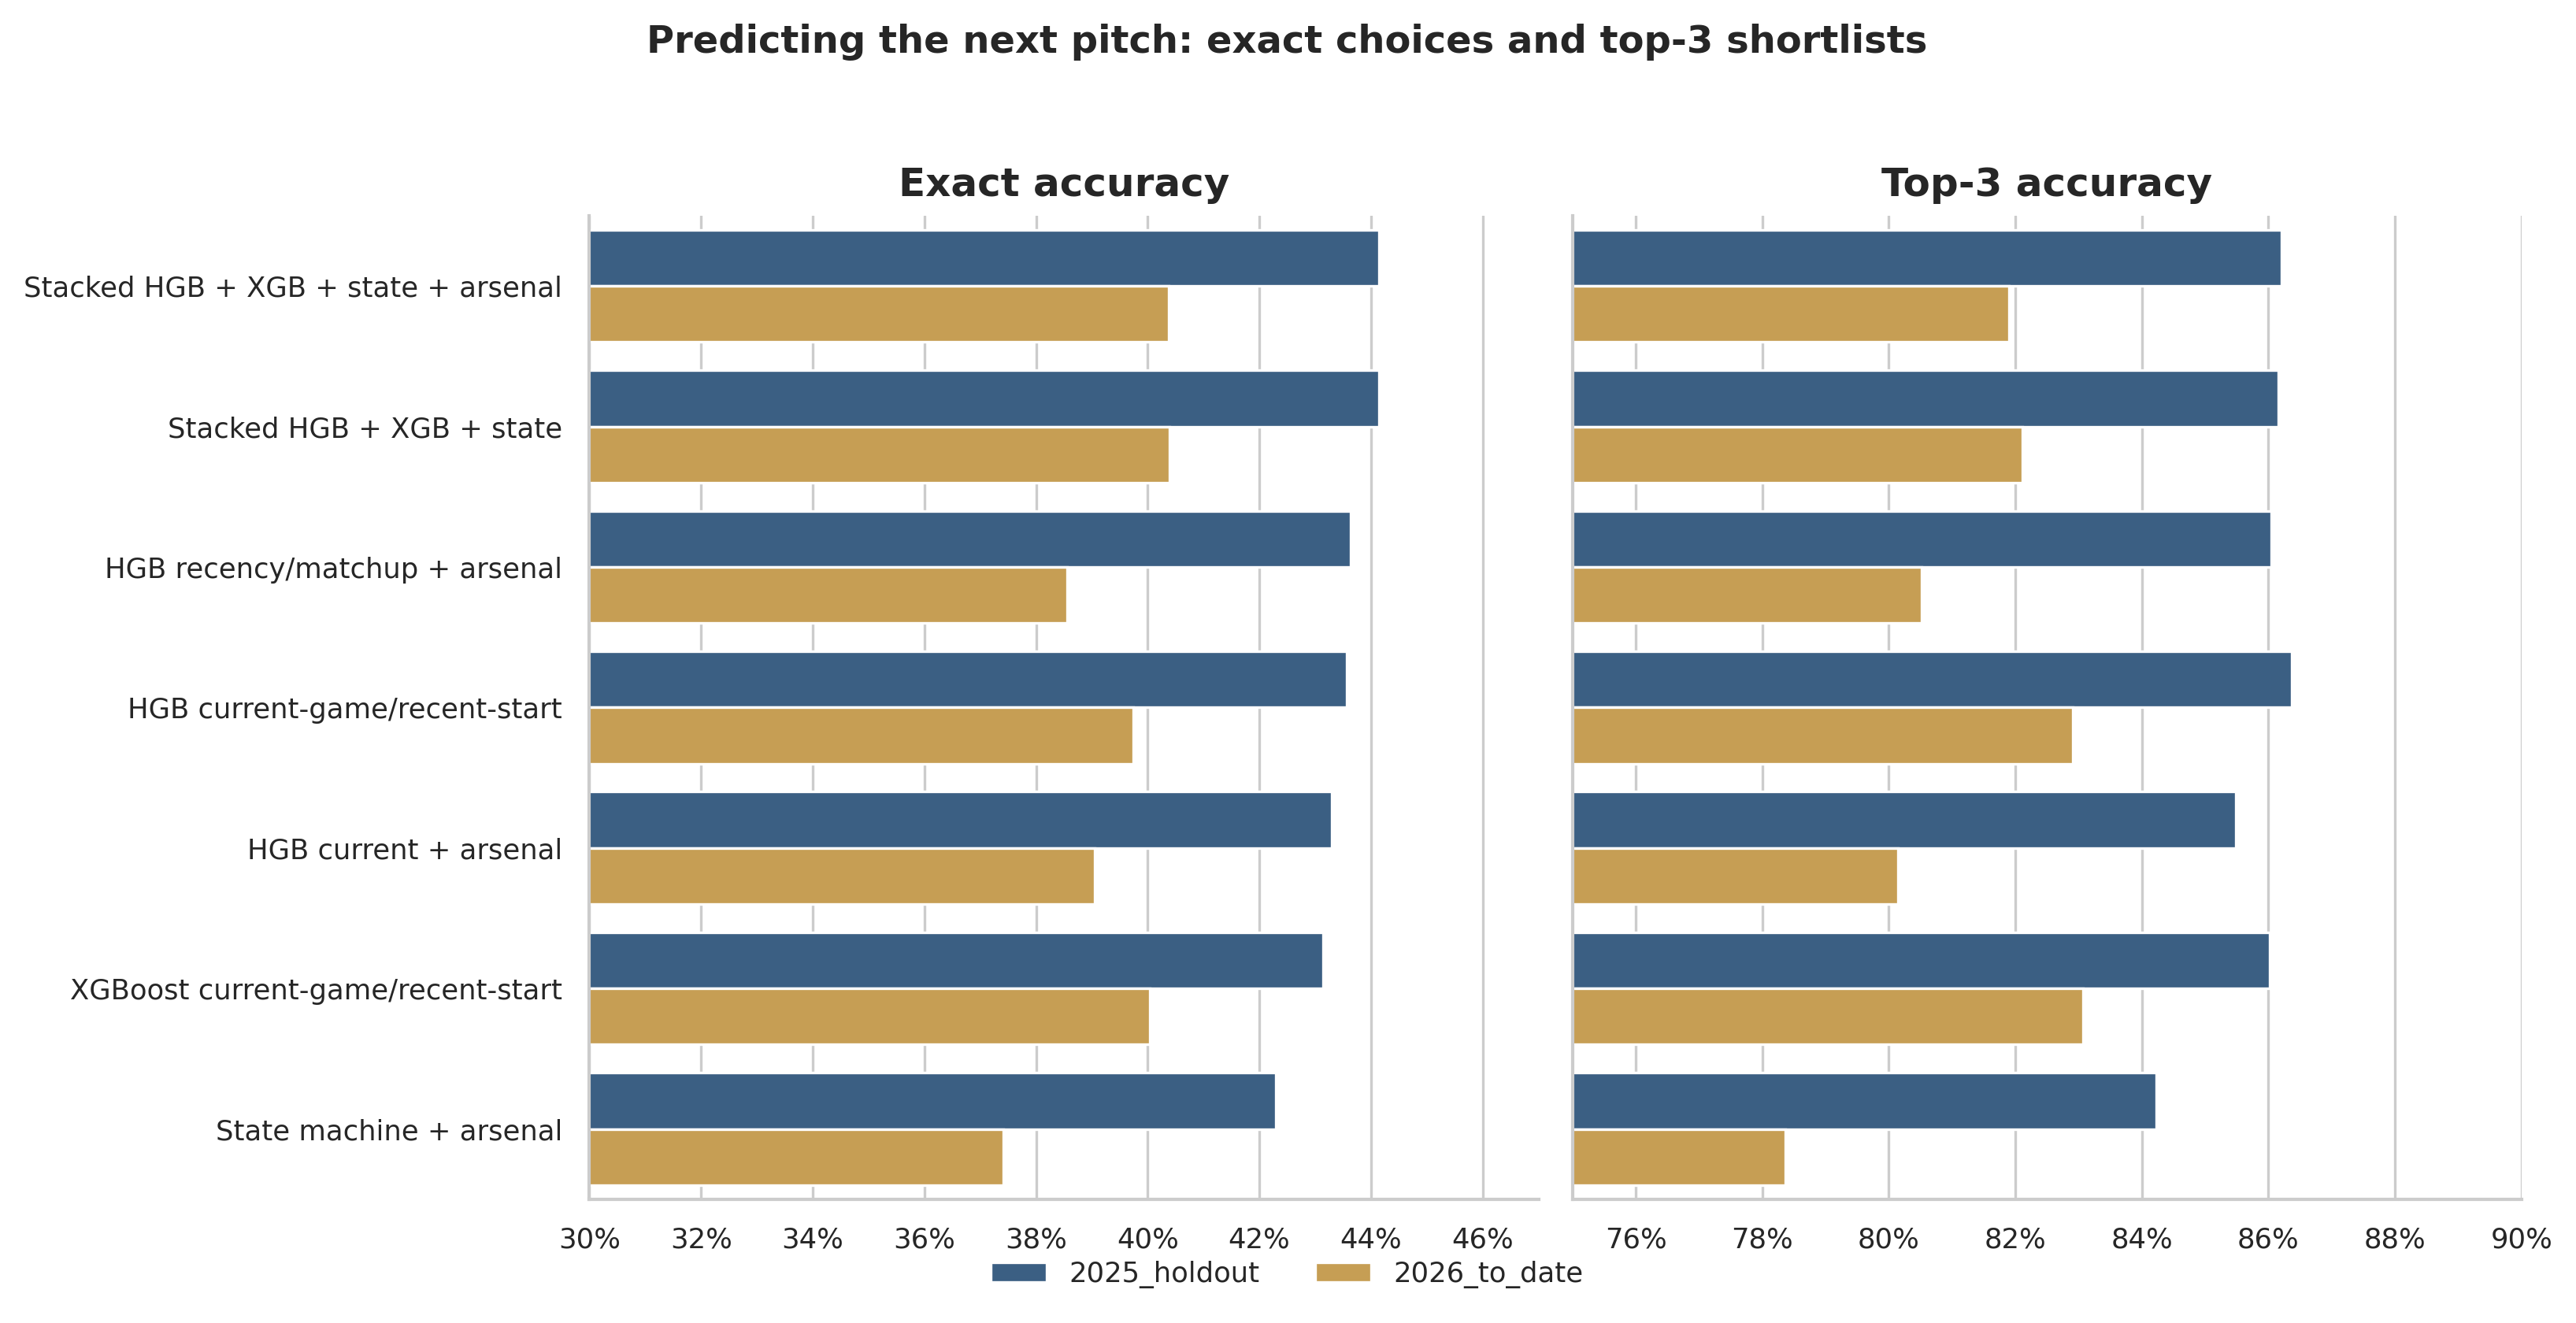
\includegraphics[width=.82\linewidth]{figures/01_model_comparison_exact_top3.png}
\caption{Predictive comparison across state-machine, boosted, XGBoost, and stacked specifications. Exact accuracy measures whether the top predicted pitch matches the pitch actually thrown. Top-three accuracy is included because pitch selection is a mixed strategy. A model can be useful if it places the actual pitch inside a small plausible set. The stacked model has the strongest exact accuracy on both the 2025 holdout and the 2026 temporal validation set.}
\label{fig:modelcomparison}
\end{figure}
\begin{table}[tbhp]
\centering
\caption{Selected model performance on held-out 2025 data and 2026 temporal validation}
\begin{tabular}{lccccc}
Model & Dataset & Rows & Exact & Top 2 & Top 3 \\
\midrule
Dummy baseline & 2025 holdout & 52,324 & 0.319 & -- & -- \\
State machine & 2025 holdout & 52,324 & 0.423 & 0.682 & 0.842 \\
Current-game HGB & 2025 holdout & 52,324 & 0.436 & 0.703 & 0.864 \\
XGBoost & 2025 holdout & 52,324 & 0.431 & 0.699 & 0.860 \\
Stacked model & 2025 holdout & 52,324 & 0.441 & 0.707 & 0.862 \\
State machine & 2026 to date & 82,282 & 0.374 & 0.622 & 0.784 \\
Current-game HGB & 2026 to date & 82,282 & 0.397 & 0.663 & 0.829 \\
XGBoost & 2026 to date & 82,282 & 0.400 & 0.666 & 0.831 \\
Stacked model & 2026 to date & 82,282 & 0.404 & 0.664 & 0.821 \\
\bottomrule
\end{tabular}
\addtabletext{HGB denotes histogram gradient boosting. The stacked model combines HGB, XGBoost, and state-machine class probabilities. Values are rounded to three decimals.}
\label{tab:models}
\end{table}

\subsection*{State context reduces uncertainty}

The state-machine results clarify why exact prediction remains difficult. Pitchers do not usually have one deterministic next pitch. However, adding context raises the share of the modal pitch and lowers entropy. At the pitcher-only level, the weighted modal pitch share is 38.2\% and weighted entropy is 2.11 bits. Adding count and previous pitch raises the weighted modal share to 44.5\% and lowers entropy to 1.88 bits. Adding batter side increases the modal share to 47.4\% and lowers entropy to 1.73 bits. The tradeoff here is sparsity meaning that the median number of pitches per state falls from more than 2,000 in pitcher-only states to 10 in pitcher-count-previous-pitch-batter-side states. The smoothing and fallback design is therefore necessary rather than cosmetic.

\begin{figure}[tbhp]
\centering
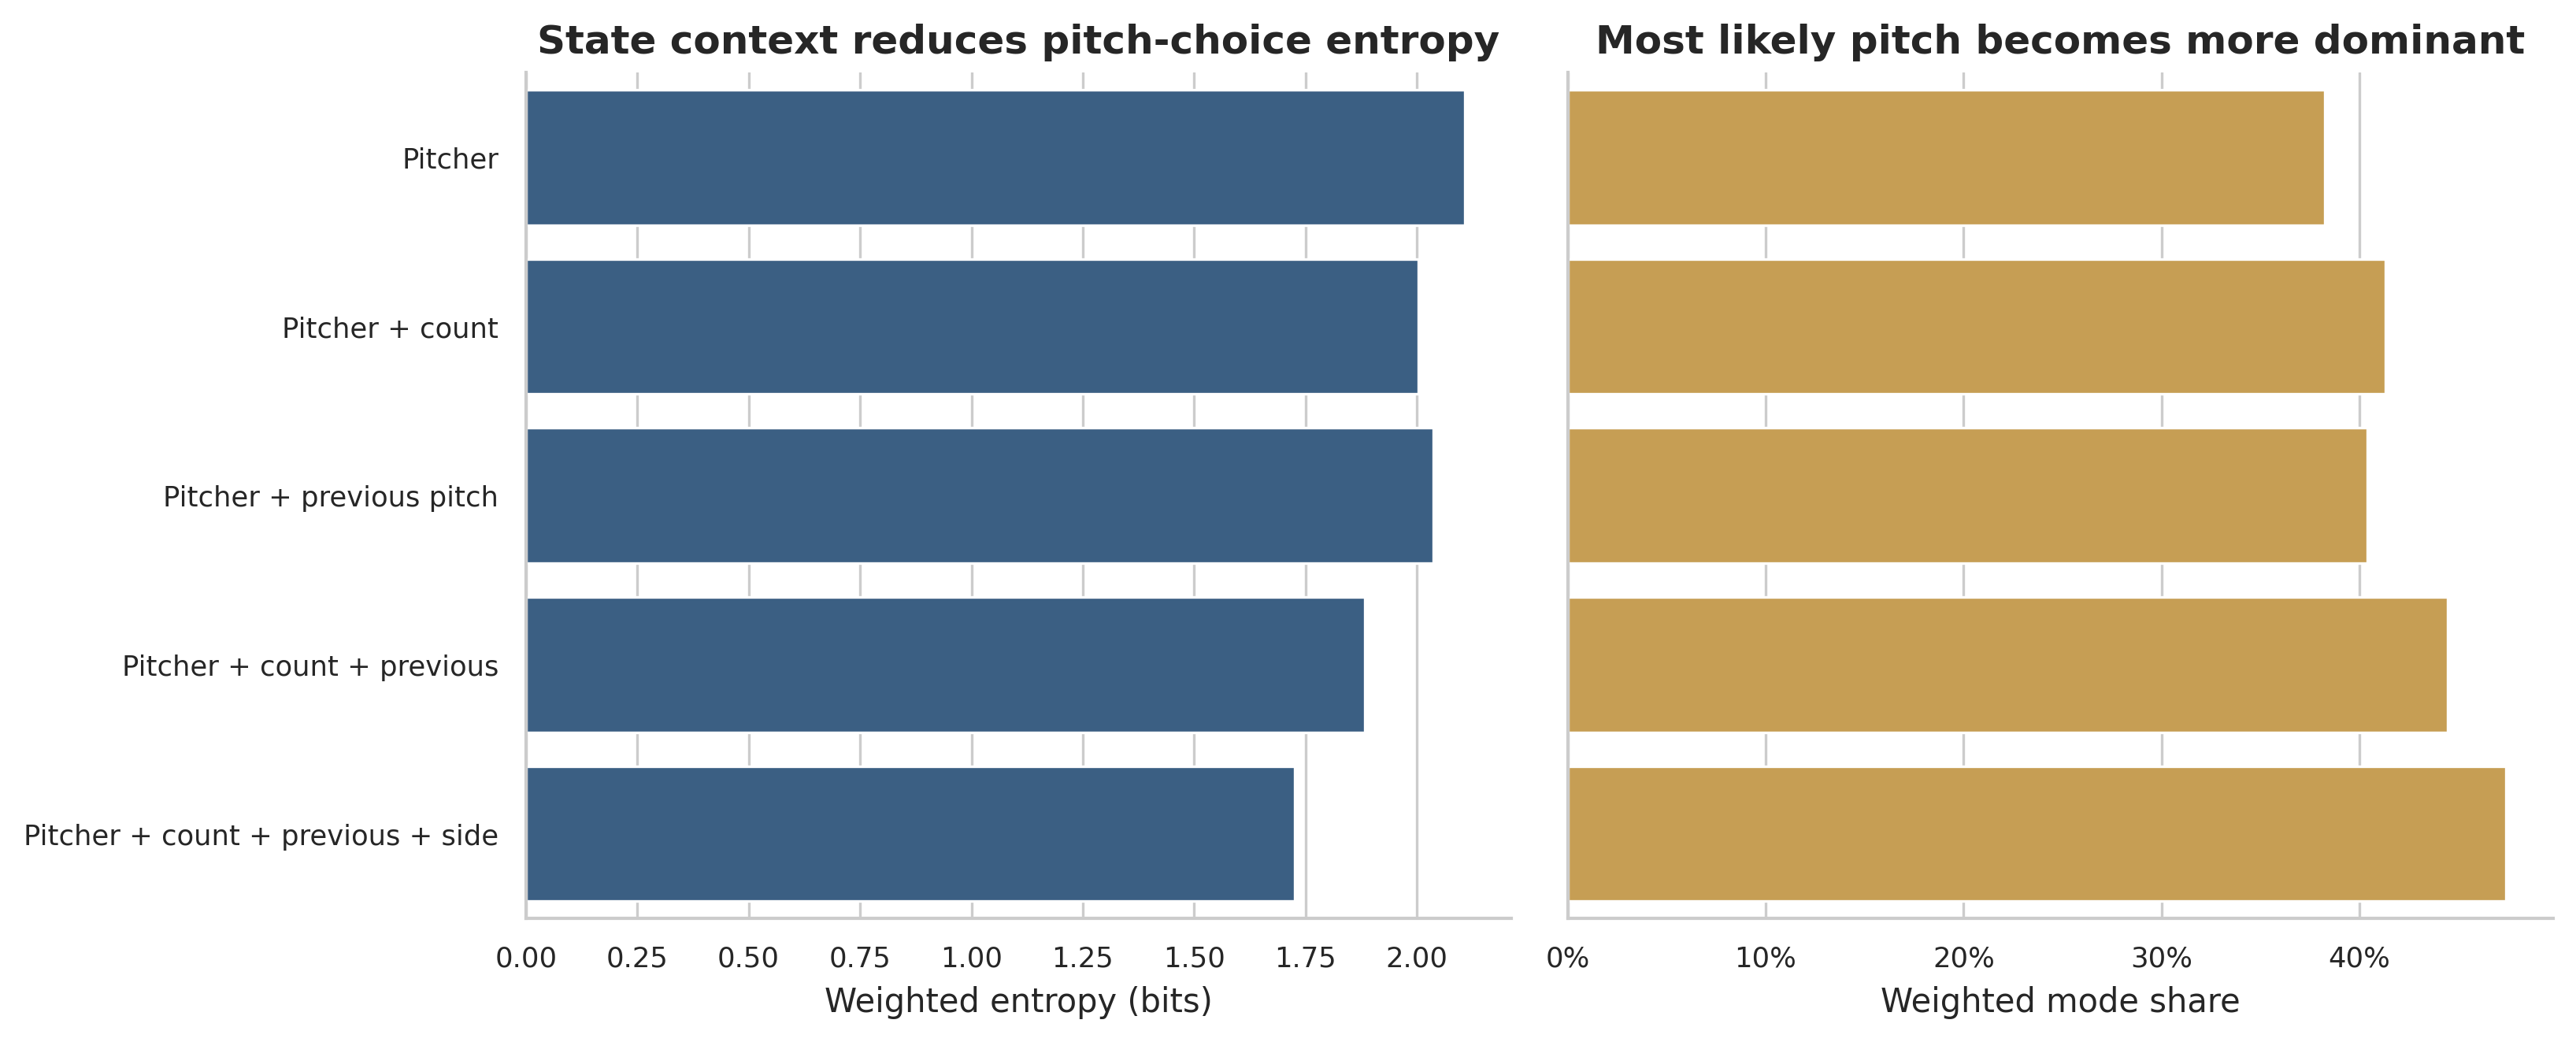
\includegraphics[width=.78\linewidth]{figures/04_state_context_entropy_mode_share.png}
\caption{Context makes pitch selection more concentrated but also more sparse. The state machine becomes more certain as it moves from pitcher-only states to pitcher-count-previous-pitch-batter-side states, but the number of observations per state declines. This motivates the use of smoothing and fallback states.}
\label{fig:entropy}
\end{figure}

\subsection*{Regression surfaces show pitcher and context structure}

The OLS beta analysis provides a compact description of repertoire and context effects. Pitcher fixed effects differ sharply across pitch types, which is expected because pitchers are constrained by their arsenals. More informative for sequence interpretation are the context coefficients: previous fastballs, sinkers, sliders, and changeups shift the next-pitch probabilities in different directions; count effects are especially visible in two-strike and three-ball counts; and batter handedness shifts pitch mix without fully determining it. These regressions are not presented as causal estimates. They are descriptive summaries of how observed pitch choices move across interpretable baseball conditions.

\begin{figure}[tbhp]
\centering
\begin{minipage}{.45\linewidth}
\centering
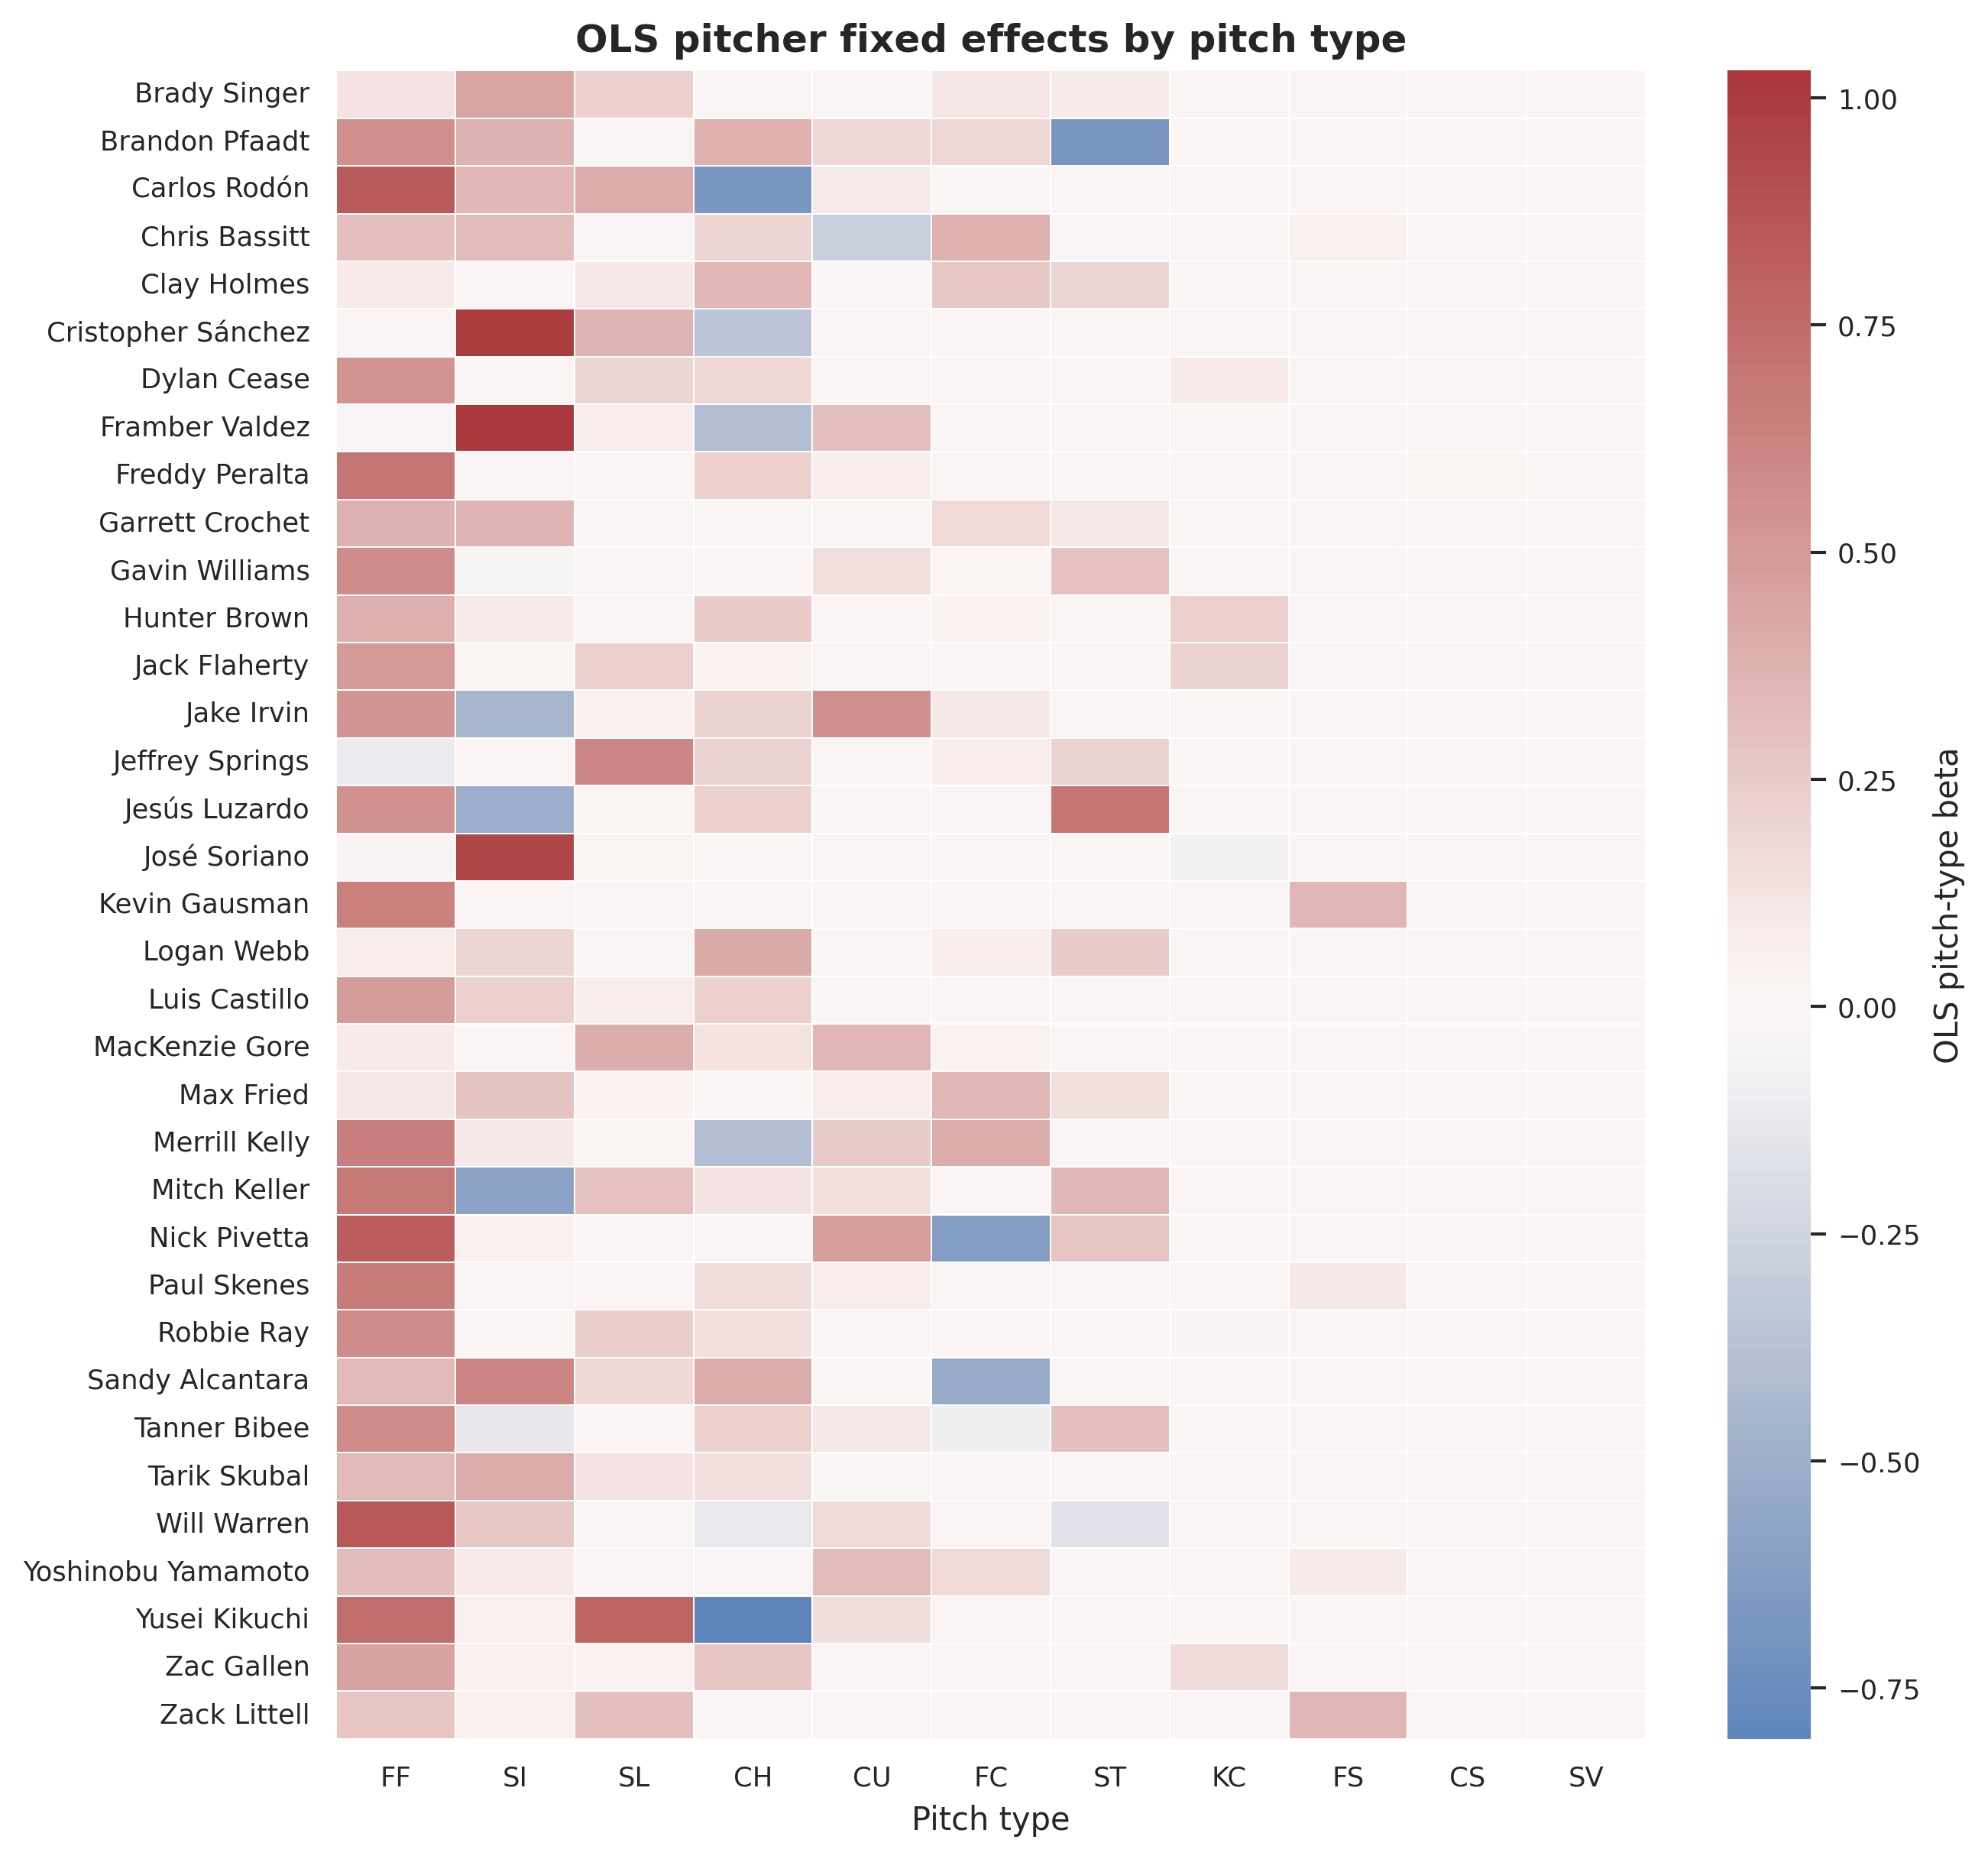
\includegraphics[width=\linewidth]{figures/08_ols_pitcher_pitch_beta_heatmap.png}
\end{minipage}
\hfill
\begin{minipage}{.45\linewidth}
\centering
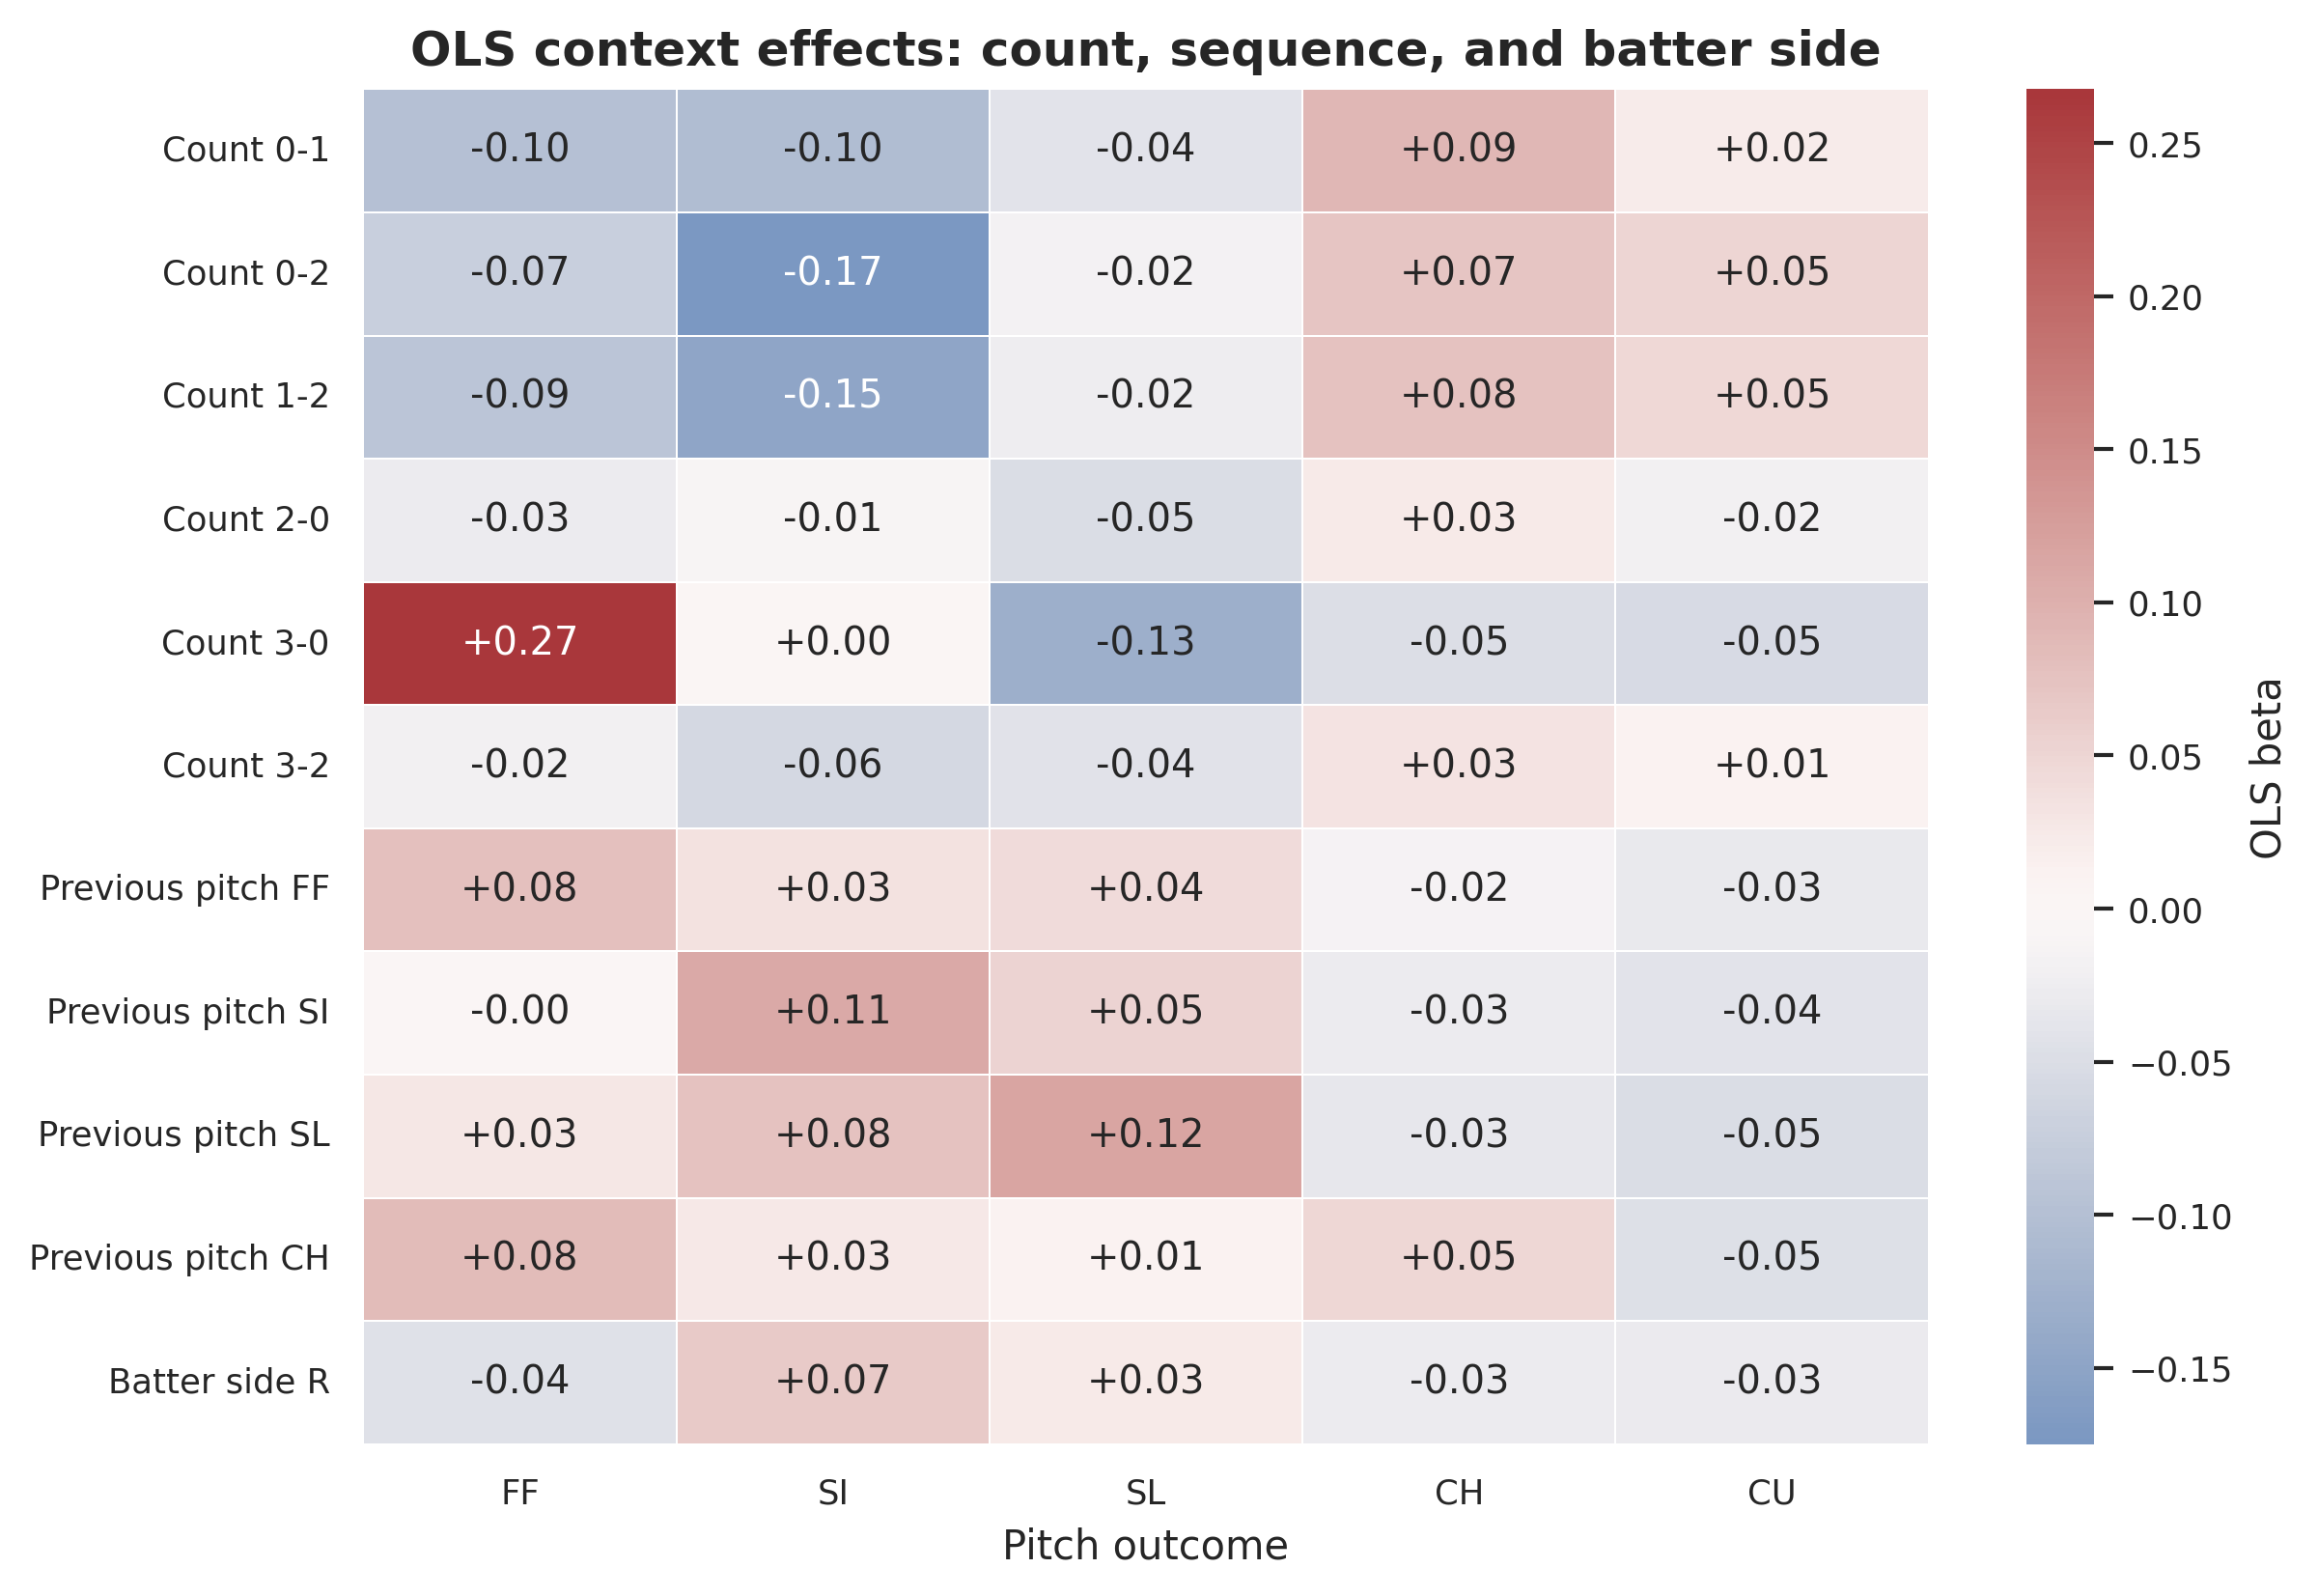
\includegraphics[width=\linewidth]{figures/09_ols_context_beta_heatmap.png}
\end{minipage}
\caption{OLS linear probability summaries. Left, pitcher-by-pitch beta coefficients show repertoire structure after accounting for observed context. Right, context beta coefficients show how count, previous pitch, and batter side shift pitch probabilities. The regression results are descriptive and are used to interpret strategic regularities rather than to claim causal pitch effects.}
\label{fig:ols}
\end{figure}

\subsection*{Grouped SHAP explains the boosted model}

Raw SHAP rankings can be misleading when player-name indicators are included. In an early interpretation, the model appeared to care heavily about four-seam fastballs and one individual pitcher. Grouping the one-hot variables gives a better reading. The largest global feature group is pitcher identity and arsenal, followed by previous pitch type, count leverage, two-pitches-ago pitch type, batter handedness, previous release speed, and previous pitch result. This pattern is consistent with the state-machine results: the model is strongest when it knows who is pitching, what that pitcher can throw, what has just been thrown, and what count pressure the pitcher faces.

\begin{figure}[tbhp]
\centering
\begin{minipage}{.45\linewidth}
\centering
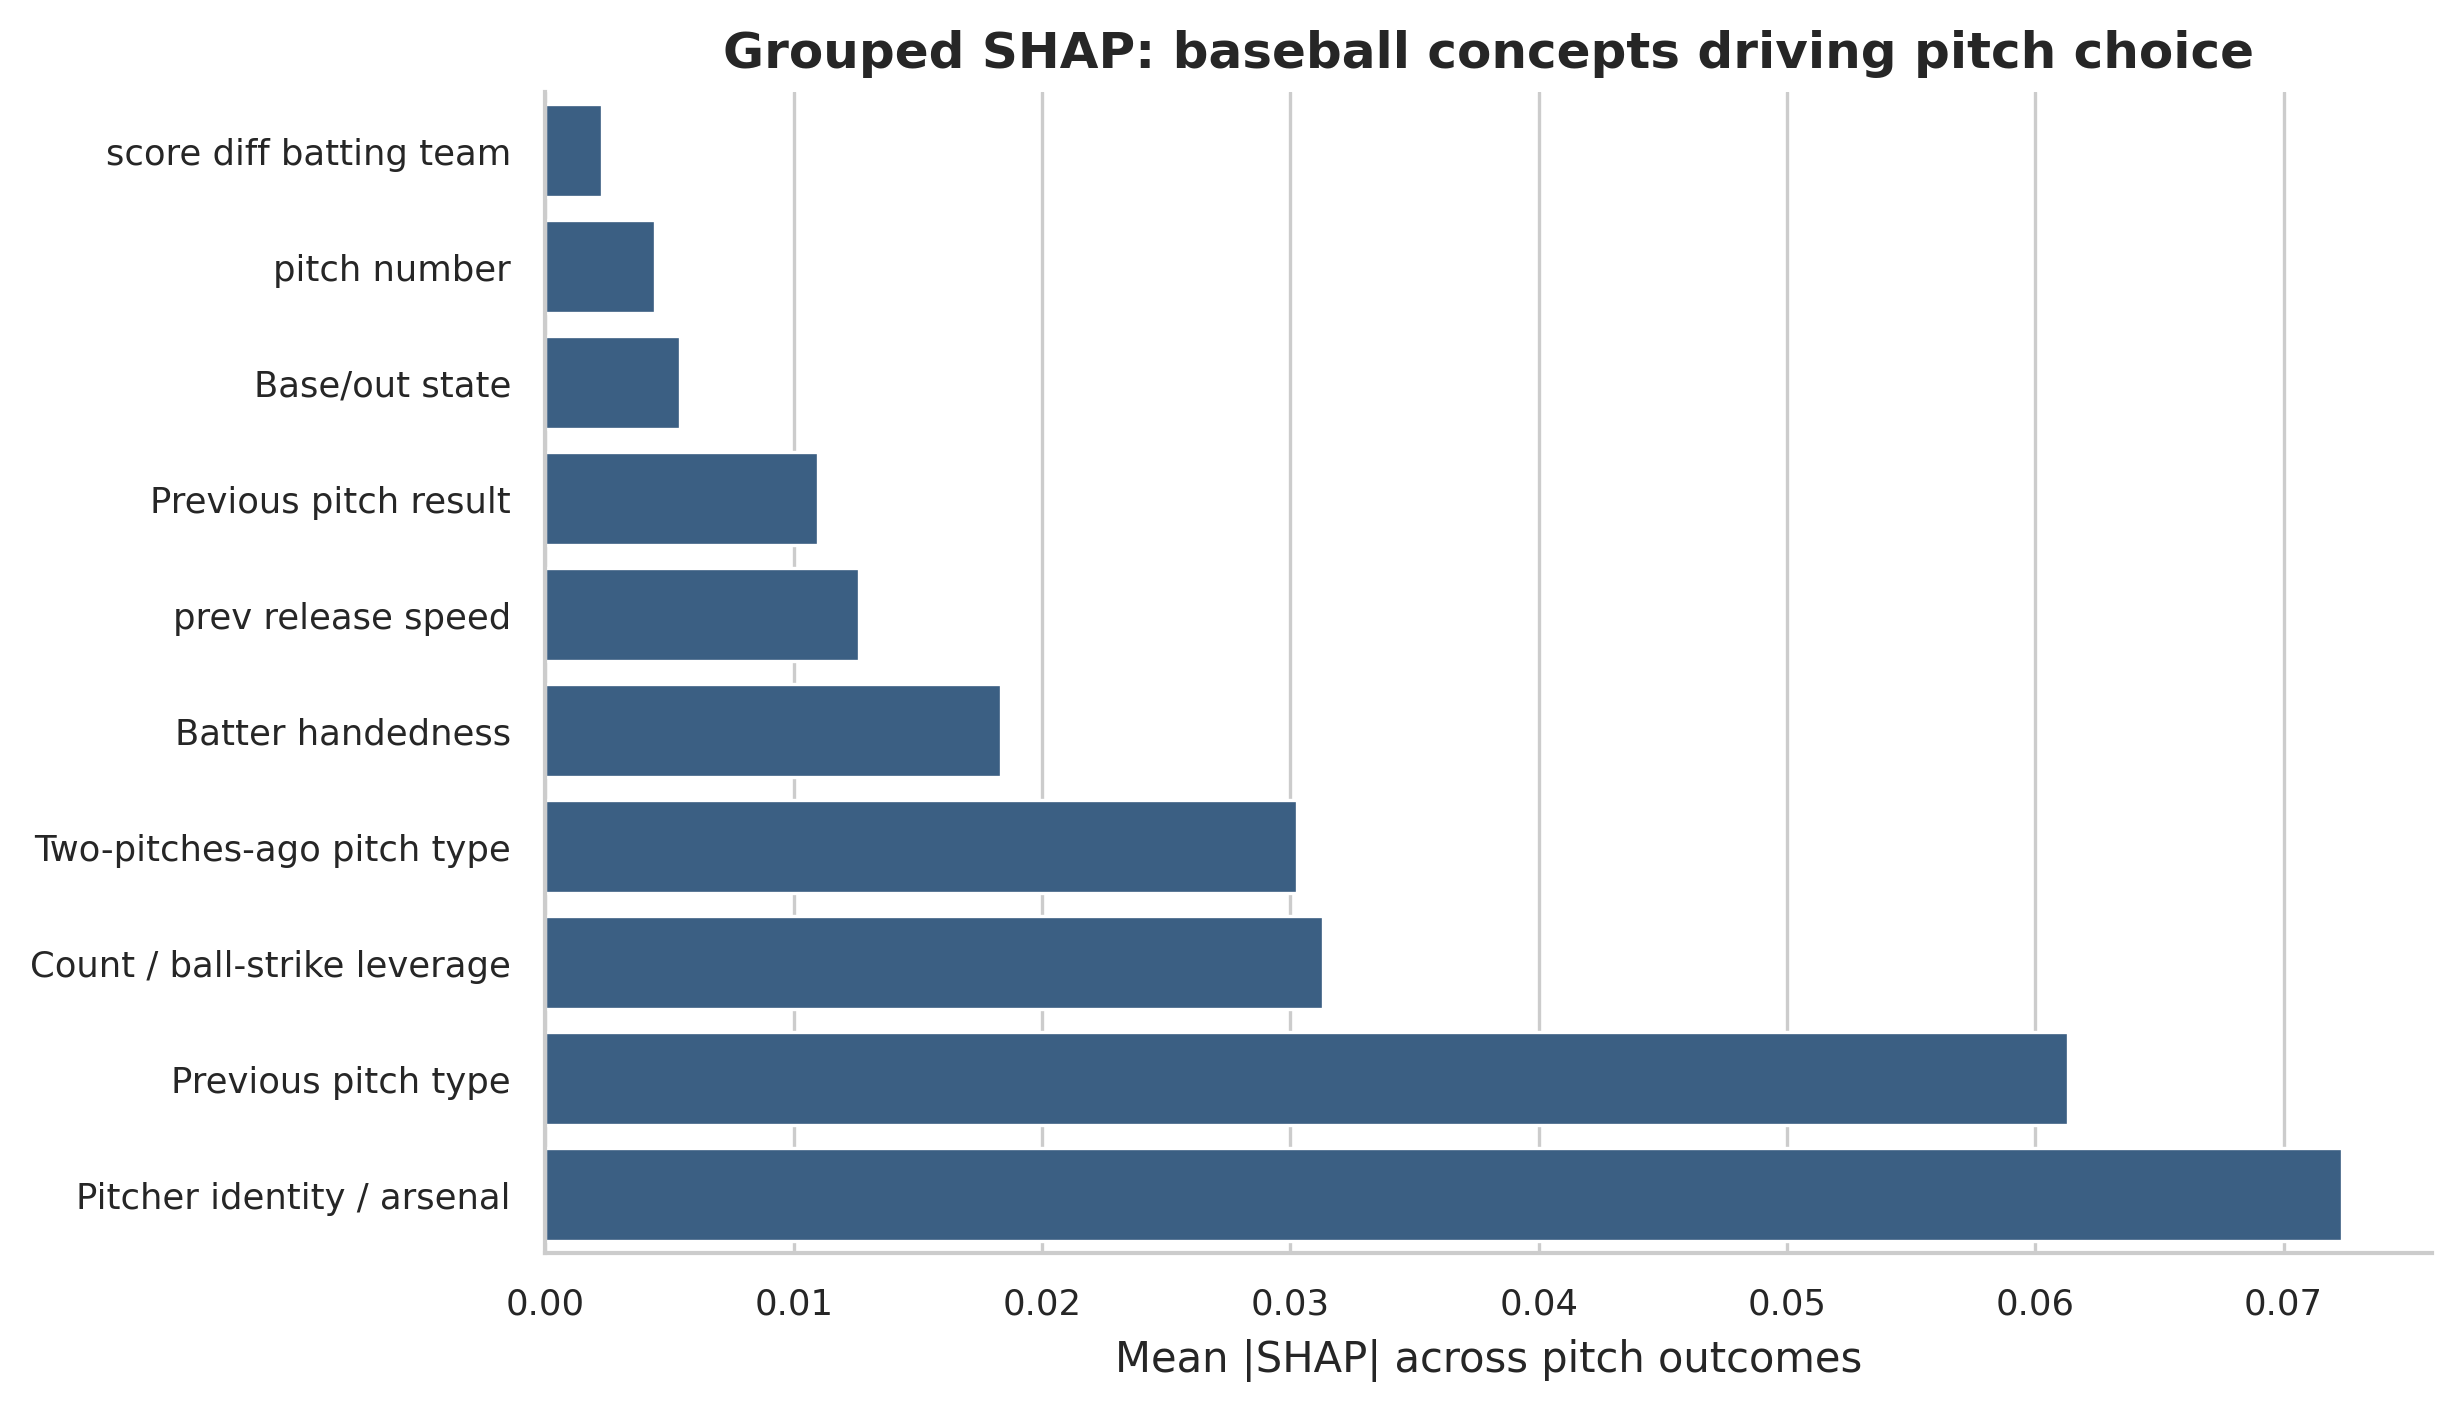
\includegraphics[width=\linewidth]{figures/11_shap_grouped_global_importance.png}
\end{minipage}
\hfill
\begin{minipage}{.45\linewidth}
\centering
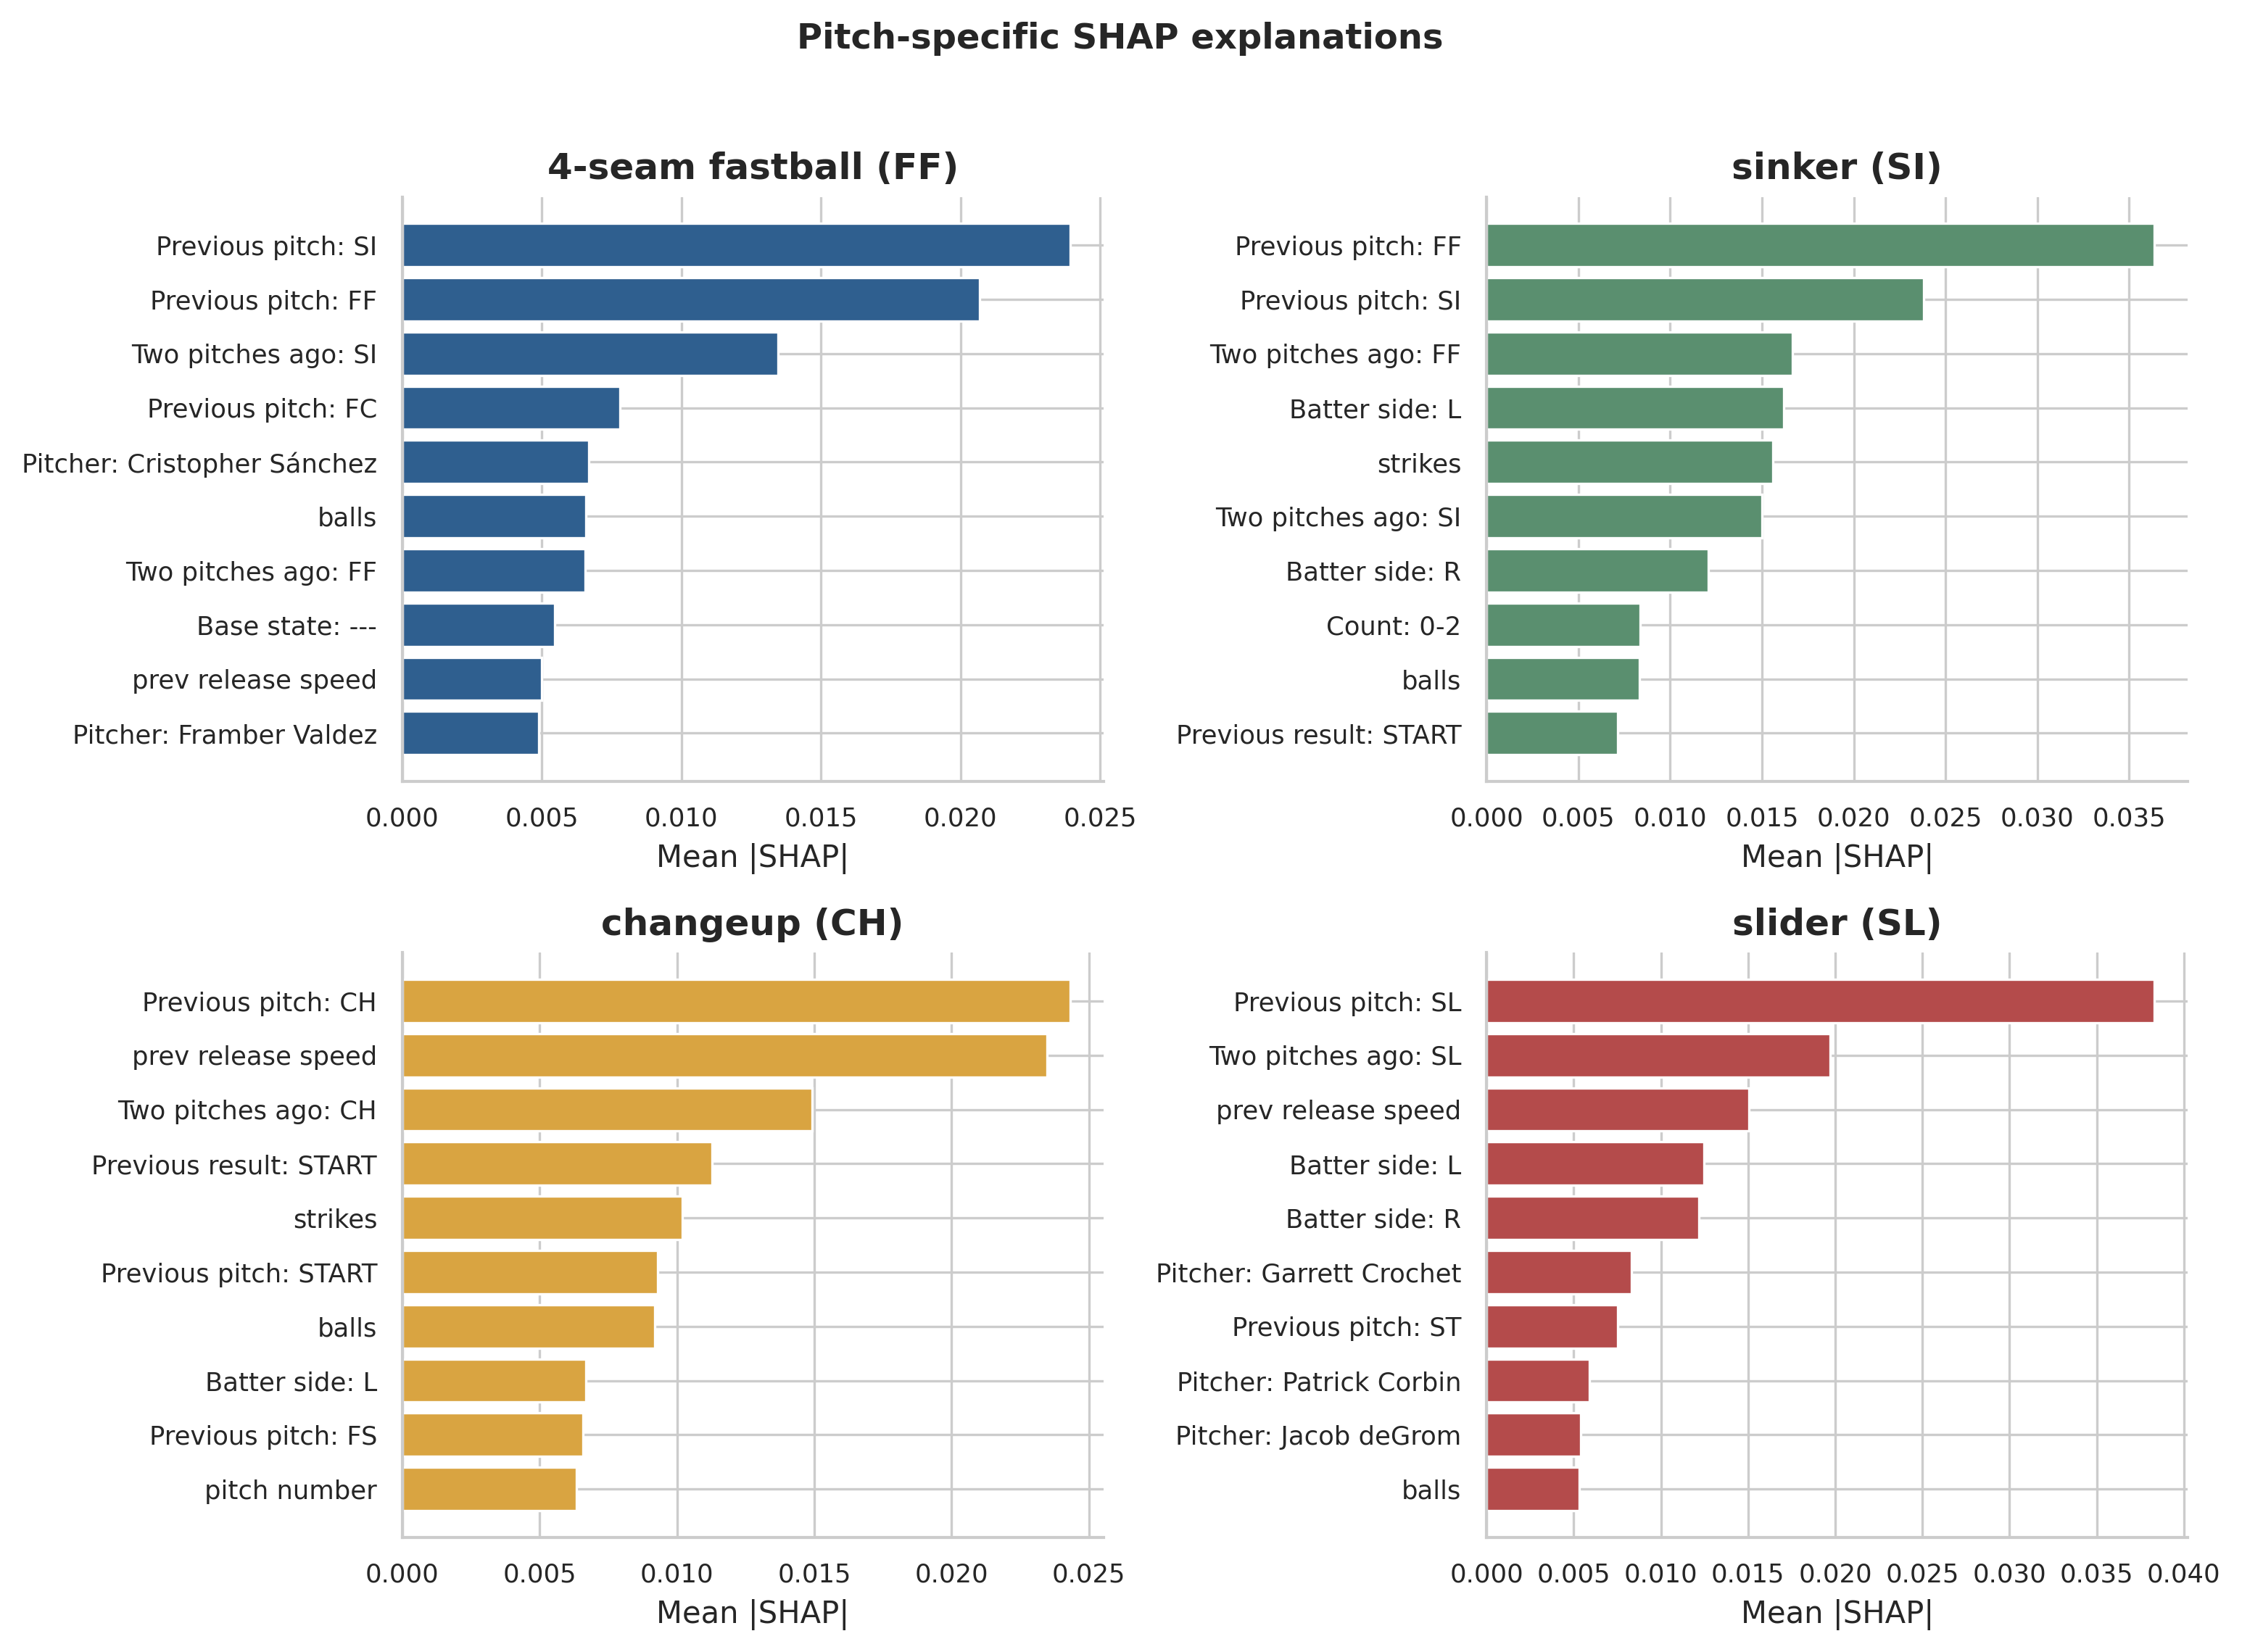
\includegraphics[width=\linewidth]{figures/12_shap_pitch_specific_panels.png}
\end{minipage}
\caption{SHAP interpretation of boosted pitch-type models. Left, one-hot features are grouped into baseball concepts to avoid over-reading individual player indicators. Right, pitch-specific panels show that the importance of recent pitch history, count, handedness, and repertoire differs by target pitch type.}
\label{fig:shap}
\end{figure}

\subsection*{Pitch transitions reveal sequence habits}

The empirical transition matrix reinforces the same conclusion from a different angle. Some transitions are common because they reflect general baseball strategy, such as alternating hard and soft pitches or returning to a primary fastball. Others are common because of selection into pitcher-specific arsenals. A transition matrix alone cannot identify intent, deception, or game theory that may occur within an MLB game. It can, however, show which pitch-pair probabilities are large enough to become useful ingredients in a predictive state model.

\begin{figure}[tbhp]
\centering
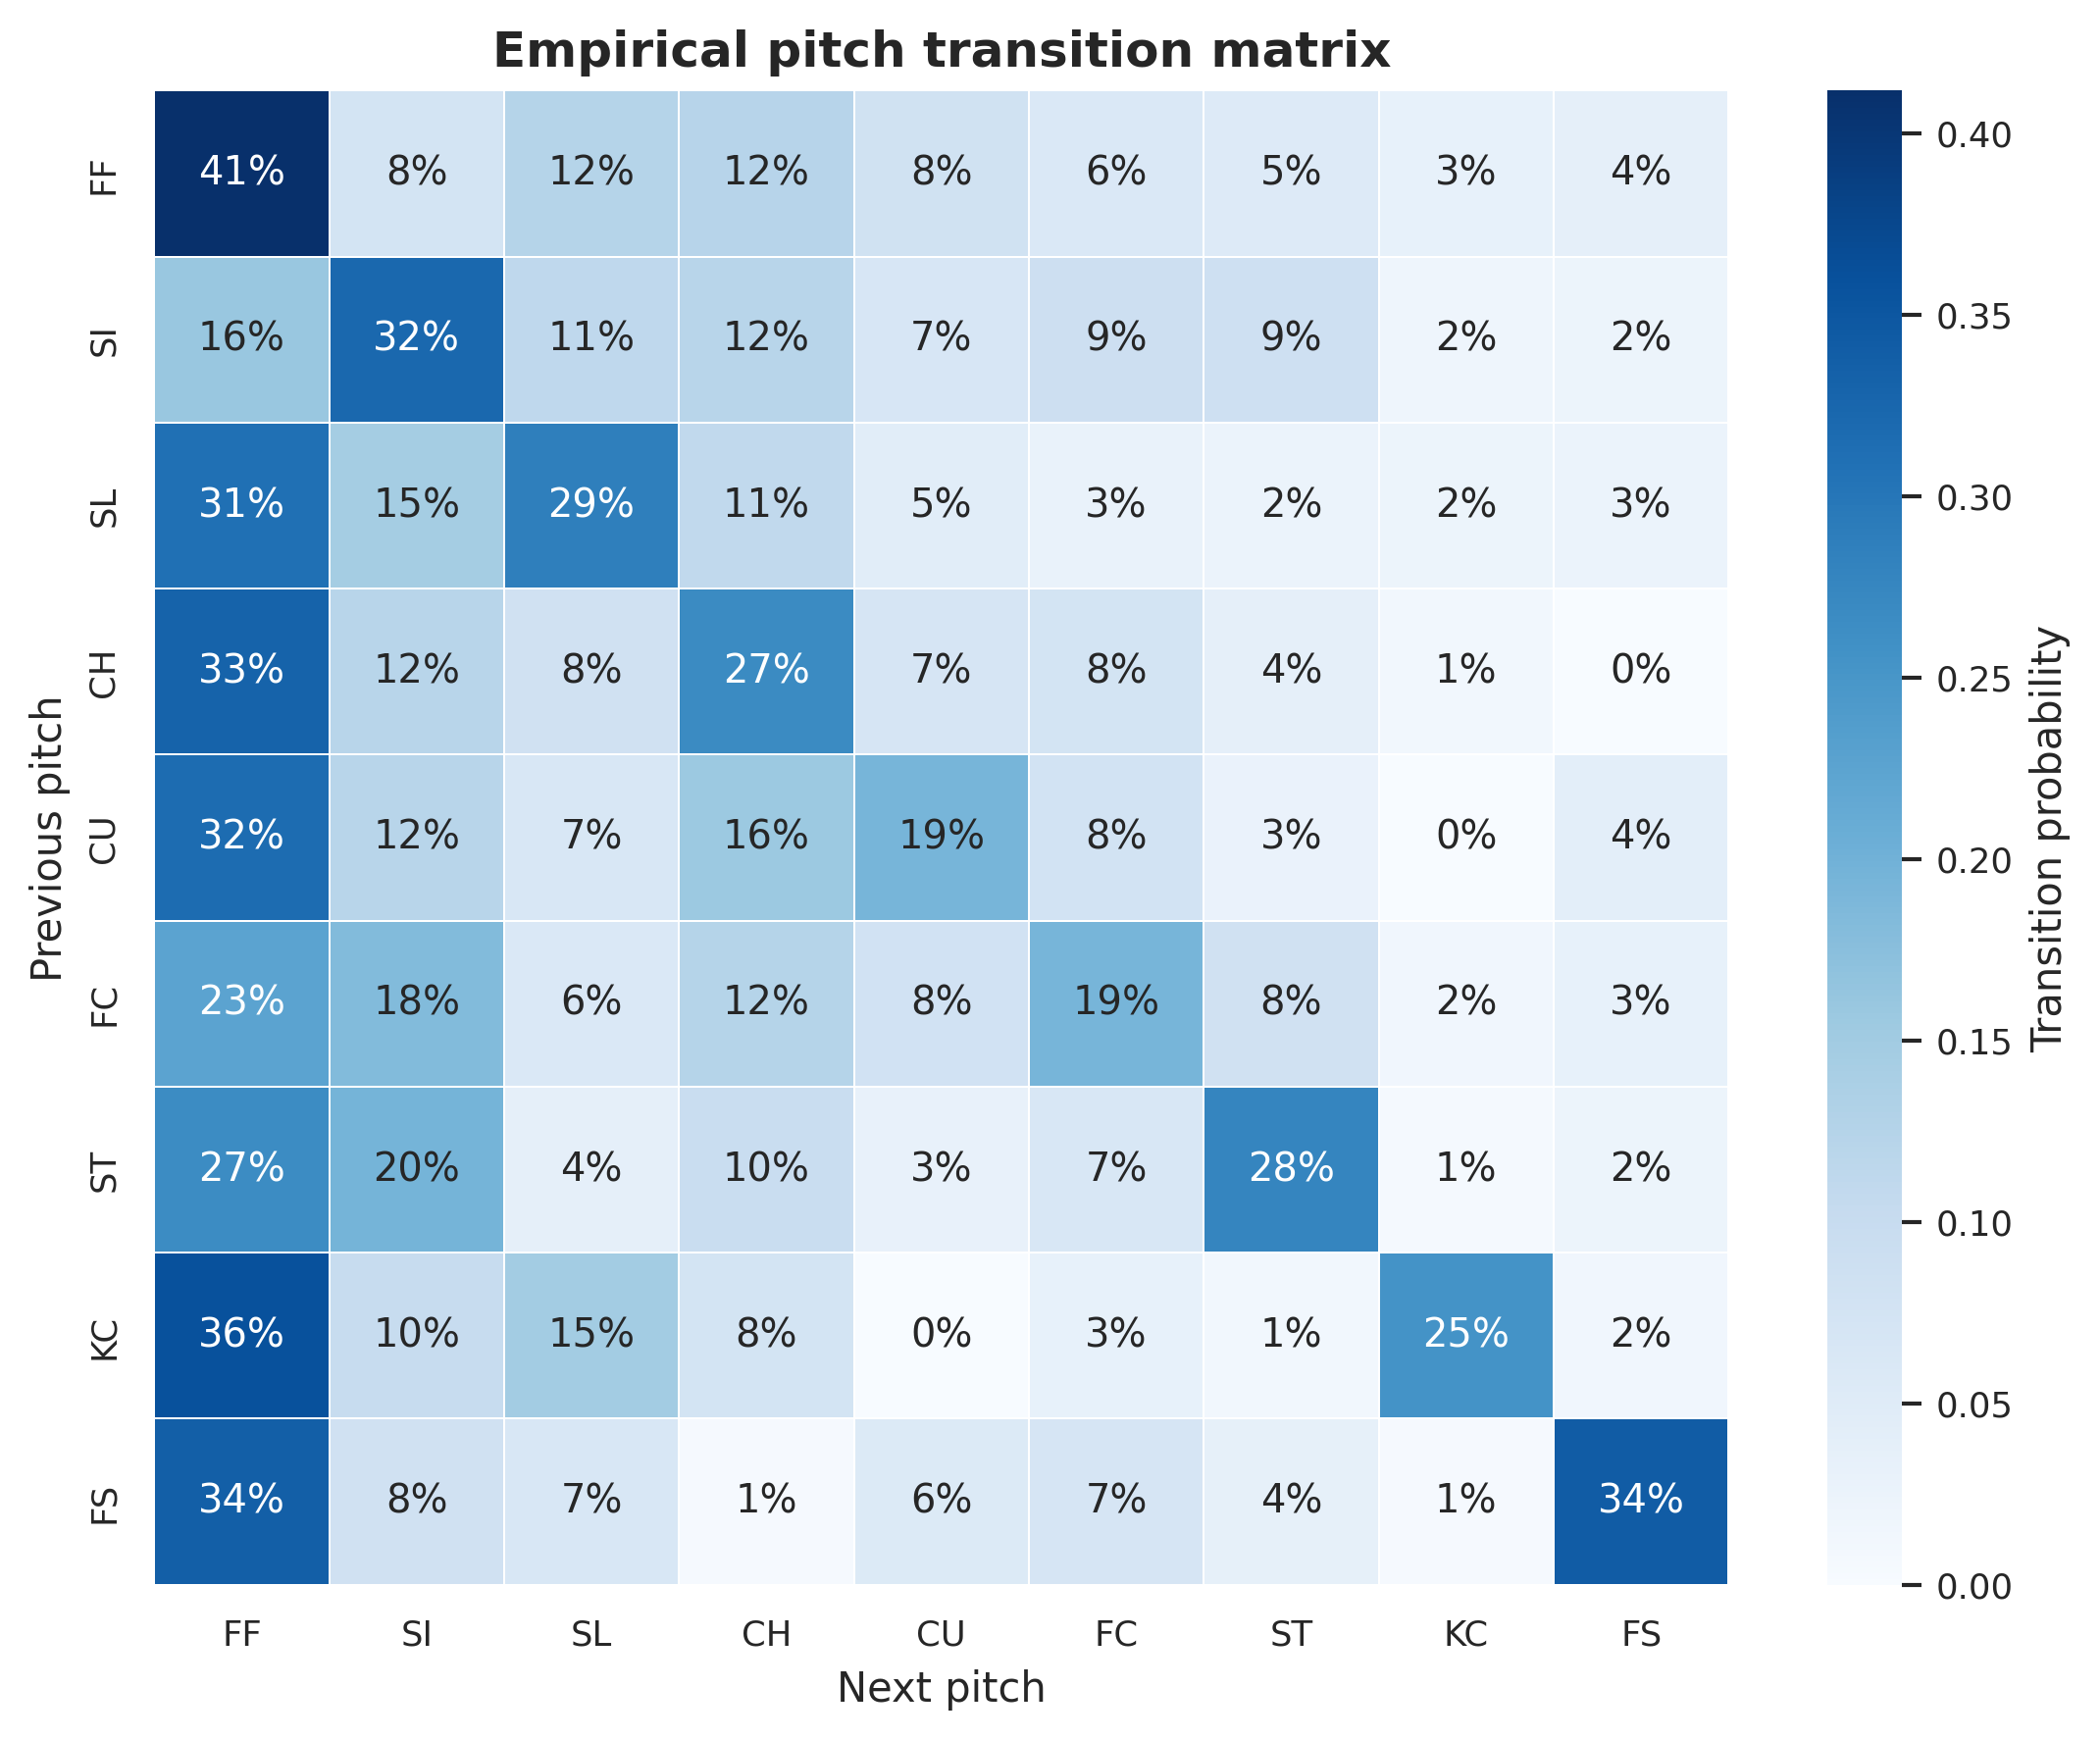
\includegraphics[width=.70\linewidth]{figures/14_pitch_transition_matrix.png}
\caption{Empirical pitch transition matrix for the 2025 training sample. Rows represent the previous pitch type and columns represent the observed next pitch type. The matrix summarizes aggregate sequencing tendencies, while the predictive state machine conditions these transitions further by pitcher, count, and batter side.}
\label{fig:transitions}
\end{figure}

\section*{Discussion}

The main finding is that pitch selection is predictable enough to model, but not predictable enough to treat as deterministic. The best model correctly identifies the exact pitch 44.1\% of the time on the 2025 holdout and 40.4\% of the time on 2026 validation. Those values are above a simple baseline, but they also leave substantial irreducible uncertainty. From an empirical experience, this makes sense in the context of baseball. Pitchers continue to iterate their pitch sequence to ensure that their pitches are unpredictable. Additionally, batters adapt, catchers and coaches influence pitch calls, and the available public data do not fully observe scouting reports, pitcher fatigue, injury status, catcher signs, or strategic deception.

The comparison between models is also informative. The state machine is less flexible than the boosted models but remains significant because it uses the right baseball state. Boosted models improve accuracy by using richer interactions and continuous context, especially current-game pitch mix, matchup history, batter history, and recent-start behavior. The stacked model adds a small gain by letting a meta-model decide when the state machine or boosted classifiers are more trustworthy. The temporal validation drop from 2025 to 2026 is expected: pitch mixes change, pitcher roles change, batters adjust, and the 2026 sample ends on June 4 rather than covering a full season.

The project has several limitations. First, the sample is restricted to high-volume pitchers, so it describes established pitchers due to the data volume rather than relievers with small samples, or pitchers returning from injury. Second, pitch-type labels are treated as the outcome, but pitch design also includes velocity, movement, location, and tunneling which are aspects of pitching that were not included in this model. Third, the model predicts observed pitch choice rather than pitch effectiveness. A stronger future version would jointly model pitch type and intended location, add catcher and umpire context, use rolling injury or velocity-change indicators, and compare CatBoost to the current HGB and XGBoost stack because CatBoost is designed to handle categorical variables directly \cite{prokhorenkova2018catboost}. Fourth, selection bias remains important: the model only observes pitches that were actually thrown in situations that actually occurred rather than looking at potential situation.

Moving forward, I would like to separate likelihood from effectiveness. In an ideal world, I would build two connected models. The first model would predict the likely pitch menu in a given state. The second model would predict the expected value of each possible pitch using outcomes such as whiff probability, called-strike probability, weak-contact probability, hard-contact risk, and expected run value. This would let the app say both, ``This pitcher is likely to throw a slider,'' and, ``The changeup may be the better option in this count against this hitter.''

I would also solve the sparse-data problem more directly. Some pitcher-batter-count states have very few observations, especially for relievers, new players, injured pitchers, and rare matchups. In an ideal version, I would use hierarchical modeling or partial pooling so that the model could borrow information from similar pitchers and hitters. For example, if one pitcher has only faced a batter a few times, the model could still learn from pitchers with similar arsenals, handedness, velocity, and sequencing patterns. This would make the model useful for more players instead of only established high-volume pitchers.

\section*{Agentic analysis}

While building the app portion of this project, I used Codex's GPT 5.5 to scaffold and build a website deployed via Vercel. Given several detailed prompts, I instructed the agent to build a website that was "beautiful, has a good UI, easy to use, and could be used by an MLB team to predict the next pitch in a baseball game." Before actually building the website, I used an agent to have a "conversation" about what I expected the website to look like. I found that this was better than giving a one-shot prompt, as demonstrated in class, letting an agent create the site, then iterating based on the output. After having an initial scaffolding for the site, I added an API with MLB schedules and upload my data via csvs that would be used for the website. The agent also helped with some of the aspects I ran into challenges with in my terminal, such as deploying the app.

I also used an agent to clean and organize my code, as well as create paper figures. The most useful contributions helped expand my dataset from 20 pitchers to 100 pitchers, implement recency-weighted HGB and XGBoost models, and learn how to set file paths for my visualization outputs.

The assistant was less reliable when interpretation required domain judgment. For example, when using it for a SHAP reading, Gemini 3 made the model look too narrow, using individual one-hot features, such as a previous four-seam fastball or one pitcher name, appear highly important. That output was technically valid but scientifically thin, and Gemini was hesitant to my rejection of that interpretation. When prompted for a stronger explanation, the final analysis grouped SHAP features into concepts such as arsenal, previous pitch type, count leverage, and batter handedness, yielding a more defensible outcome. 

This experience changed the workflow in two ways. First, the assistant made it easier to scale experiments, produce visualizations, and build a website, but the agents were still poor without human judgment. Second, the assistant exposed how easy it is to confuse a predictive signal with an explanation. A model can use a pitcher's name because it summarizes a pitcher's arsenal, role, and team strategy, but this does not mean the pitcher's name itself explains a pitch. My final paper therefore is using AI assistance extensively to accelerate my project's data analysis and website product, but requires significant questioning and a high level of curiosity. The accepted outputs are those that survived code review and questions about code, temporal validation, and frankly, a high level of baseball knowledge and interpretation.

\href{https://docs.google.com/document/d/1mokZbiQgp-POLGlgpM5lacJ6LA4XFGBKIqMvBdzO-j0/edit?usp=sharing}{AI Transcript Link}

\dataavail{All code, processed outputs, notebooks, and visualizations are intended for release in a public GitHub repository. The repository will contain numbered notebooks, a code directory, a data directory or cloud-data link, and an output directory. Raw pitch-level data are publicly available from Baseball Savant. Processed tables and scripts used to reproduce the analyses will be included with the final course repository when public release is complete.}

\acknow{The author thanks the course instructor for feedback that sharpened the modeling design, especially the recommendation to compare pitcher-specific loops, pooled boosted models, state-machine probabilities, and regression beta analysis.}

\begin{thebibliography}{14}

\bibitem{baseballsavant}
Major League Baseball, Baseball Savant Statcast search. Available at https://baseballsavant.mlb.com/statcast\_search. Accessed 14 May 2026.

\bibitem{pybaseball}
J. LeDoux, Pybaseball: Python package for baseball data acquisition and analysis. Available at https://github.com/jldbc/pybaseball. Accessed 14 May 2026.

\bibitem{hamilton2014pitch}
M. Hamilton, P. Hoang, L. Layne, J. Murray, D. Padgett, C. Stafford, H. Tran, Applying machine learning techniques to baseball pitch prediction. In \textit{Proceedings of the 3rd International Conference on Pattern Recognition Applications and Methods} (ICPRAM, 2014), pp. 520--527.

\bibitem{sidle2018multiclass}
G. Sidle, H. Tran, Using multi-class classification methods to predict baseball pitch types. \textit{Journal of Sports Analytics} \textbf{4}, 85--93 (2018).

\bibitem{lee2022pitch}
J. S. Lee, Prediction of pitch type and location in baseball using ensemble model of deep neural networks. \textit{Journal of Sports Analytics} \textbf{8}, 115--126 (2022).

\bibitem{lin2025pitchtype}
Z.-H. Lin, K.-C. Wu, Pitch type prediction in MLB: A machine learning and deep learning approach. \textit{Advances in Transdisciplinary Engineering} (2025). https://doi.org/10.3233/ATDE251162.

\bibitem{augustine2024pitchpredictor}
M. Augustine, MLB Pitch Predictor: Using machine learning to predict pitch sequencing. \textit{Medium} (2024). Available at https://medium.com/@MichaelAugustine78/mlb-pitch-predictor-using-machine-learning-to-previse-pitch-sequencing-c5d38b9ac97c.

\bibitem{norris1998markov}
J. R. Norris, \textit{Markov Chains} (Cambridge University Press, Cambridge, UK, 1998).

\bibitem{wooldridge2010econometric}
J. M. Wooldridge, \textit{Econometric Analysis of Cross Section and Panel Data} (MIT Press, Cambridge, MA, ed. 2, 2010).

\bibitem{friedman2001greedy}
J. H. Friedman, Greedy function approximation: A gradient boosting machine. \textit{Ann. Stat.} \textbf{29}, 1189--1232 (2001).

\bibitem{chen2016xgboost}
T. Chen, C. Guestrin, XGBoost: A scalable tree boosting system. In \textit{Proceedings of the 22nd ACM SIGKDD International Conference on Knowledge Discovery and Data Mining} (Association for Computing Machinery, New York, NY, 2016), pp. 785--794.

\bibitem{lundberg2017unified}
S. M. Lundberg, S.-I. Lee, A unified approach to interpreting model predictions. In \textit{Advances in Neural Information Processing Systems} \textbf{30} (2017), pp. 4765--4774.

\bibitem{prokhorenkova2018catboost}
L. Prokhorenkova, G. Gusev, A. Vorobev, A. V. Dorogush, A. Gulin, CatBoost: Unbiased boosting with categorical features. In \textit{Advances in Neural Information Processing Systems} \textbf{31} (2018), pp. 6638--6648.

\bibitem{james1984abstract}
B. James, \textit{The Bill James Baseball Abstract 1984} (Ballantine Books, New York, NY, 1984).

\end{thebibliography}

\end{document}